\documentclass[11pt,reqno]{amsart}

\usepackage{amsmath,amssymb,amsthm}
\usepackage[margin=1.1in]{geometry}
\usepackage{microtype}
\usepackage{tikz}
\usepackage[colorlinks=true,linkcolor=blue,citecolor=blue]{hyperref}

\theoremstyle{plain}
\newtheorem{theorem}{Theorem}[section]
\newtheorem{proposition}[theorem]{Proposition}
\newtheorem{lemma}[theorem]{Lemma}
\newtheorem{corollary}[theorem]{Corollary}
\theoremstyle{definition}
\newtheorem{remark}[theorem]{Remark}
\newtheorem{example}[theorem]{Example}

\newcommand{\R}{\mathbb{R}}
\newcommand{\Z}{\mathbb{Z}}
\newcommand{\C}{\mathbb{C}}
\newcommand{\HH}{\mathbb{H}}
\newcommand{\SU}{\mathrm{SU}(2)}
\newcommand{\SO}{\mathrm{SO}(3)}
\newcommand{\Pin}{\mathrm{Pin}(2)}
\newcommand{\tr}{\operatorname{tr}}
\newcommand{\Inat}{I^{\natural}}
\newcommand{\gr}{\operatorname{gr}}
\newcommand{\Sig}{\Sigma}
\newcommand{\pill}{\mathcal{P}}
\newcommand{\bp}{\mathfrak{b}}

\begin{document}

\title[Traceless characters and instanton gradings for $2$-bridge and $(3,n)$ knots]
{Traceless $\SU$ characters and $\Z/4$ instanton gradings\\ for two-bridge and $(3,n)$-torus knots}

\author{Bernd J. Wuebben}
\subjclass[2020]{57R58 (primary); 57K10, 57K31, 53D40, 58J30 (secondary)}
\keywords{Instanton knot homology, traceless character varieties,
pillowcase, Atiyah--Floer conjecture, two-bridge knots, torus knots,
binary dihedral representations, spectral flow}
\date{First version: July 27, 2026. This version: August 15, 2026}

\begin{abstract}
For the $(3,n)$-torus knots we determine the $\Z/4$ gradings of the reduced singular instanton chain
complex through the double branched cover $\Sigma(2,3,n)$ rather than through an index computation:
each irreducible flat connection on the cover has two traceless knot lifts of equal grading, so
Daemi--Scaduto's theorem for the irreducible torus-knot complex transports to a grading split. For $n$
odd this recovers the chain-rank distribution $(1+a,a,a,a)$, $a=-\sigma/4$, conjectured by
Poudel--Saveliev and established for all torus knots by Daemi--Scaduto. Comparing that rank vector with
$\operatorname{rank}\Inat=\|\Delta\|_1$ then determines the total rank of the framed differential in
every residue class of $n$ modulo $6$: it vanishes for $n\equiv1,2$ and equals one for $n\equiv4,5$.
The comparison uses no index theory, which is what carries it into the even classes, where
$\Sigma(2,3,n)$ is not a homology sphere; $T(3,8)$ is a non-alternating knot with vanishing framed
differential. Along the way we prove that every irreducible traceless $\SU$ character of a two-bridge
knot is binary-dihedral, with the traceless Riley polynomial in closed form, and that for the
$(3,n)$-torus knots exactly $(\det-1)/2$ characters are dihedral, so for $n$ odd none is; and we
identify the first nonzero pillowcase differential, for $8_{19}=T(3,4)$, as a corner figure-eight
bigon absent on two-bridge knots.
\end{abstract}

\maketitle

\section{Introduction}

\subsection{The Atiyah--Floer conjecture and its knot version}
Let $Y$ be a closed oriented $3$-manifold with a Heegaard splitting $Y=Y_0\cup_\Sigma Y_1$. Two Floer
theories attach to this picture. On the gauge-theoretic side is Floer's instanton homology
$HF^{\mathrm{inst}}(Y)$, generated by flat $\SU$ connections and with a differential counting
anti-self-dual instantons on $Y\times\R$. On the symplectic side, the moduli space $M(\Sigma)$ of flat
$\SU$ connections on $\Sigma$ is symplectic, the handlebodies determine Lagrangians $L_0,L_1\subset
M(\Sigma)$, and one forms the Lagrangian Floer homology $HF^{\mathrm{symp}}(L_0,L_1)$. The Atiyah--Floer
conjecture~\cite{Atiyah} asserts these are isomorphic (for a recent survey of the Lagrangian Floer
theory in which the conjecture sits, see Auroux~\cite{Auroux}). The one general theorem is the
mapping-torus case
of Dostoglou--Salamon~\cite{DS}; the Heegaard-splitting statement remains open, obstructed by the
singularities of $M(\Sigma)$ and by figure-eight bubbling in the adiabatic limit.

There is a knot-theoretic analogue in which the pillowcase plays the role of $M(\Sigma)$. Let
$K\subset S^3$ be a knot, and cut $S^3$ along a Conway sphere meeting $K$ in four points into two
$2$-string tangles. A representation $\rho\colon\pi_1(S^3\setminus K)\to\SU$ is \emph{traceless} if every
meridian maps to a traceless element (conjugate to $\operatorname{diag}(i,-i)$); this is the boundary
condition of Kronheimer--Mrowka's singular instanton theory~\cite{KM1,KM2}. Restricting traceless flat
connections of each tangle to the four-punctured sphere and applying holonomy perturbations, one obtains
immersed Lagrangians $L_0,L_1$ in the \emph{pillowcase}
\[
\pill=(\R/2\pi\Z)^2/\iota,\qquad \iota(\gamma,\theta)=(-\gamma,-\theta),
\]
the traceless $\SU$ character variety of the four-punctured sphere: a two-sphere with four $\Z/2$
orbifold points~\cite{Lin,HHK1}. The \emph{knot Atiyah--Floer conjecture} of Hedden--Herald--Kirk and
Cazassus--Herald--Kirk--Kotelskiy~\cite{HHK1,CHKK} asserts that a bounding-cochain-deformed Lagrangian
Floer homology of $(L_0,L_1)$ is isomorphic, as a relatively $\Z/4$-graded group, to the reduced
singular instanton knot homology $\Inat(K)$. (A \emph{bounding cochain} is a formal combination of
self-intersection points of an immersed Lagrangian that deforms the Floer differential by
higher-polygon counts --- the standard device by which Lagrangian Floer theory absorbs disk bubbling
\cite{Auroux,CHKK}; \emph{figure-eight bubbling} is the degeneration of holomorphic strips, specific
to immersed Lagrangians, that makes the correction necessary here \cite{CHKK}.)

\subsection{Purpose and scope}
Two things here are new. The first is a determination of the $\Z/4$ grading distribution for the
$(3,n)$-torus knots that runs through the double branched cover rather than through an index
calculation: the two traceless knot lifts of a flat connection on $\Sig(2,3,n)$ carry the same
grading, so Daemi--Scaduto's theorem for the irreducible torus-knot complex transports to a
grading split, and hence to the rank vector of the framed complex. The second is that comparing that
rank vector with $\|\Delta\|_1$ determines the total rank of the framed differential in \emph{all
four} residue classes of $n$ modulo $6$, including the even classes, where the Fintushel--Stern index
is unavailable because $\Sig(2,3,n)$ is not a homology sphere. Both are collected in
Theorem~\ref{thm:C}.

Around them the paper makes explicit, for two tractable infinite families, the
representation-theoretic data on which the pillowcase construction rests: the traceless character
variety (the generators), the $\Z/4$ spectral-flow gradings, and the differential. The same data is
in active use beyond the pillowcase program: Dai--Mallick--Taniguchi have recently used an explicit
analysis of the traceless character varieties of two-bridge knots to compute, in part, symmetry
actions on their singular instanton complexes~\cite{DMT}.

Three explicit verifications are reported below: the exact-arithmetic check of Theorem~\ref{thm:A},
the counts of Proposition~\ref{prop:count}, and the gradings of Section~\ref{sec:grading}. They are carried
out by short computer programs, included as ancillary files with this preprint and also available at
the public repository \url{https://github.com/bwuebben/pillowcase-bounding-cochain}. Each re-derives
its output by an independent route; the first works in exact Gaussian-integer arithmetic.

\subsection{Results}\label{sec:intro-results}
Section~\ref{sec:pillow} records the pillowcase and the traceless characters as generators.
Section~\ref{sec:2bridge} proves:

\begin{theorem}[Traceless characters of two-bridge knots are dihedral]\label{thm:A}
Let $K=\bp(p,q)$ be the two-bridge knot of fraction $p/q$, so $p=\det K$. Every irreducible traceless $\SU$ representation of
$\pi_1(S^3\setminus K)$ is binary-dihedral. There are exactly $(p-1)/2$ of them: writing $\omega$ for
the meridian-pair angle (the angle between the axes of two chosen meridians, the conjugacy invariant
of Section~\ref{sec:pillow}), they occur at
$\cos\omega=\cos(2\pi k/p)$ for $k=1,\dots,(p-1)/2$, independent of $q$; equivalently the traceless
Riley polynomial in $u=2\cos\omega-2$ is
\[
\phi_p(u)=\prod_{k=1}^{(p-1)/2}\Bigl(u+4\sin^2\tfrac{\pi k}{p}\Bigr),
\]
monic of degree $(p-1)/2$, with integer coefficients, $\phi_p(0)=p=\det K$, and root-sum $-p$.
\end{theorem}

We then explain (Section~\ref{sec:2bridge-pillow}) how Theorem~\ref{thm:A} clarifies the
Hedden--Herald--Kirk two-bridge isomorphism and localizes the obstruction, and we correct a naive
expectation about the earring correspondence.

Section~\ref{sec:3n} computes the $(3,n)$-torus knot characters and proves:

\begin{theorem}[Dihedral dichotomy for $(3,n)$-torus knots]\label{thm:B}
Let $n\ge2$ and $\gcd(3,n)=1$. The irreducible traceless $\SU$ characters of $T(3,n)$ are in bijection with the
traceless arcs of Section~\ref{sec:3n} (the arcs of irreducible characters that
contain a traceless point), one per arc. Exactly $(\det-1)/2$ of them are
binary-dihedral: one if $n$ is even $(\det=3)$ and none if $n$ is odd $(\det=1)$. In particular, for $n$
odd every irreducible traceless character of $T(3,n)$ is non-dihedral.
\end{theorem}

Section~\ref{sec:grading} passes to the double branched cover $\Sig(2,3,n)$ and proves the main
result of the paper. Write $C_*(K)$ for the irreducible singular instanton complex and
$\widetilde C(K)=C_*(K)\oplus C_{*-1}(K)\oplus\Z_{(0)}$ for the framed complex of the $S$-complex
of~\cite[Def.~3.21]{DSEquiv}, whose homology is $\Inat(K)$; this is not the framed instanton homology
$I^{\#}$ of a closed three-manifold. Subscripts on $\Z$ denote gradings and superscripts denote
ranks. Besides the differential $d$ of $C_*$, the differential $\widetilde\partial$ of $\widetilde C$
has a map $v\colon C_*\to C_{*-2}$ and two maps $\delta_1\colon C_1\to\Z$, $\delta_2\colon\Z\to C_{-2}$
to and from the reducible summand. For torus knots $d$ vanishes, so all of the content of
Theorem~\ref{thm:C} lies in $v,\delta_1,\delta_2$.

\begin{theorem}[Gradings and the framed differential for $(3,n)$-torus knots]\label{thm:C}
Let $\gcd(3,n)=1$ and put $a=-\sigma(T(3,n))/4$. For $n$ odd, the irreducible flat $\SO$ connections
on $\Sig(2,3,n)$ split evenly between the $\Z/4$ gradings $\mu=1$ and $\mu=3$, and
\[
\widetilde C(T(3,n))=(1+a,\,a,\,a,\,a)
\]
as a rank vector in gradings $0,1,2,3$. For every $n$ coprime to $3$, the total rank of the
differential of $\widetilde C(T(3,n))$ is
\[
\operatorname{rank}\widetilde\partial=
\begin{cases}0,& n\equiv1,2\pmod 6,\\ 1,& n\equiv4,5\pmod 6.\end{cases}
\]
In particular $T(3,8)$ has vanishing framed differential although it is non-alternating.
\end{theorem}

Theorem~\ref{thm:C} is Propositions~\ref{prop:split} and~\ref{prop:even} below.
Section~\ref{sec:819} reproduces the $8_{19}$ differential and identifies its geometric source.
Section~\ref{sec:open} states the genuinely open geometric direction.

\subsection{Strategy}
The arguments are short and largely independent, and we sketch them here.

Theorem~\ref{thm:A} is a two-sided count. Irreducible binary-dihedral representations are
automatically traceless, which produces at least $(p-1)/2$ traceless characters; the traceless
specialization $s=i$ of Riley's polynomial has $u$-degree at most $(p-1)/2$, which produces at most
that many. The bounds coincide, so the two sets are equal and the roots can be read off.

Theorem~\ref{thm:B} turns on a trace obstruction. Writing $\pi_1(S^3\setminus T(3,n))=\langle x,y\mid
x^3=y^n\rangle$, the trace of $\rho(x)$ is $\pm1$, so $\rho(x)$ cannot lie in the reflection coset of
$\Pin$; irreducibility then forces $\rho(y)$ into that coset, where every element is traceless, and
that is possible only when $n$ is even. The converse is an explicit construction.

Theorem~\ref{thm:C} has two halves, proved by different means. For the grading split we do not
evaluate an index. Daemi--Scaduto compute the irreducible torus-knot complex: it is supported in
gradings $1$ and $3$ with $a$ generators in each and vanishing differential. The branched-cover
correspondence sends each irreducible flat connection on $\Sig(2,3,n)$ to a free pair of traceless
knot lifts, and the two lifts carry the same grading; so the $a$ cover connections must divide
$a/2$ and $a/2$ between $\mu=1$ and $\mu=3$, and framing turns that into the rank vector. One step
needs care: Daemi--Scaduto and Poudel--Saveliev normalize their gradings against different reference
points, and the two differ by $\sigma\bmod4$, which vanishes here because $\sigma=-4a$. Evaluating
the Fintushel--Stern index and the equivariant $\rho$-invariant directly then serves as an
independent check, for all odd $n\le43$, rather than as the proof.

For the differential we compare two independently computed numbers. For $n$ odd the chain rank is
$1+4a$, from the first half; for $n$ even it is instead $2N+1$, since the irreducible complex then has
one generator per traceless character and Proposition~\ref{prop:count} counts those. The homology rank is pinned to $\|\Delta_{T(3,n)}\|_1$ by squeezing $\Inat$ between
Kronheimer--Mrowka's Alexander lower bound and the reduced Khovanov upper bound, the latter computed
from Sch\"utz's Bar--Natan chain decomposition for three-braids. Since
$\dim H=\dim C-2\operatorname{rank}\partial$, the difference of the two numbers \emph{is} twice the
differential rank. Nothing in that comparison uses the index, which is why it survives into the even
classes, where $\Sig(2,3,n)$ has nontrivial reducibles and the index formula does not exist.

\subsection{Three kinds of statement}
We are careful throughout to separate:
\begin{itemize}
\item[(i)] results proved here (self-contained, though some are surely classical);
\item[(ii)] classical facts and standing theorems (attributed);
\item[(iii)] computations reproduced from~\cite{HHK2,PS,Anvari} (attributed, and independently checked
where possible).
\end{itemize}
Theorem~\ref{thm:A} belongs to (i) but is elementary and essentially classical, and we say so again
where it is proved. We claim no new theorem about the knot Atiyah--Floer conjecture itself: for
two-bridge knots that is a theorem of Hedden--Herald--Kirk~\cite{HHK1,HHK2}, and for the torus knots
we treat the instanton side and the character-variety side, not the analytic identification of the
two.

\subsection*{Acknowledgements}
The literature computations reproduced here are due to Hedden--Herald--Kirk~\cite{HHK1,HHK2},
Cazassus--Herald--Kirk--Kotelskiy~\cite{CHKK}, Poudel--Saveliev~\cite{PS}, and Anvari~\cite{Anvari};
we have tried to attribute each precisely.

\section{The pillowcase and traceless characters}\label{sec:pillow}

We work with $\SU$ as the unit quaternions. An element is traceless iff it is a purely imaginary unit
quaternion (eigenvalues $\pm i$, squaring to $-1$); as a rotation it is a rotation by $\pi$. The
traceless elements form a $2$-sphere $S\subset\operatorname{Im}\HH\cong\R^3$.

\begin{proposition}[Classical; cf.~\cite{Lin,HHK1}]\label{prop:pillow}
The traceless $\SU$ character variety of the four-punctured sphere is the pillowcase
$\pill=(\R/2\pi\Z)^2/\iota$, with four $\Z/2$ orbifold points at $(\gamma,\theta)\in\{0,\pi\}^2$ and the
symplectic form descending from $d\gamma\wedge d\theta$.
\end{proposition}

\begin{proof}[Sketch]
Write $\pi_1$ of the four-punctured sphere as
$\langle X_1,\dots,X_4\mid X_1X_2X_3X_4=1\rangle$ with each $X_i\in S$. Since purely imaginary units
satisfy $X_i^{-1}=-X_i$, the relation gives $X_1X_2=X_4X_3=:A$. For pure imaginary units,
$X_iX_j=-\langle X_i,X_j\rangle+X_i\times X_j$, so when $A\neq\pm1$ its axis is well defined; equating the
two expressions for $A$ forces the four $X_i$ to be coplanar, orthogonal to $\operatorname{axis}(A)$.
Placing that axis along $k$ and writing $X_m=\cos\beta_m\,i+\sin\beta_m\,j$, the relation becomes
$\beta_2-\beta_1=\beta_3-\beta_4$; gauge-fixing $\beta_1=0$ and setting $\gamma=\beta_2$,
$\theta=\beta_4$ leaves two parameters, and the residual conjugation by the $\pi$-rotation about $i$ acts
by $(\gamma,\theta)\mapsto(-\gamma,-\theta)$. The four fixed points are the reducible (collinear)
characters.
\end{proof}

\begin{figure}[ht]
\centering
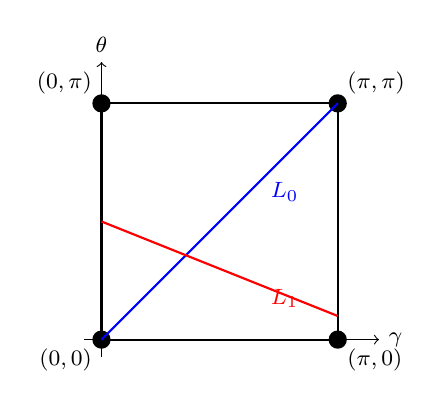
\begin{tikzpicture}[scale=1.5]
  \draw[thick] (0,0) rectangle (2,2);
  \foreach \x/\y in {0/0,2/0,0/2,2/2}{\fill (\x,\y) circle (2.2pt);}
  \node[below left] at (0,0) {\footnotesize $(0,0)$};
  \node[below right] at (2,0) {\footnotesize $(\pi,0)$};
  \node[above left] at (0,2) {\footnotesize $(0,\pi)$};
  \node[above right] at (2,2) {\footnotesize $(\pi,\pi)$};
  \draw[->] (-0.15,0)--(2.35,0) node[right] {\footnotesize $\gamma$};
  \draw[->] (0,-0.15)--(0,2.35) node[above] {\footnotesize $\theta$};
  % two rational-slope Lagrangians of a 2-bridge knot
  \draw[blue,thick] (0,0)--(2,2);
  \draw[red,thick] (0,1)--(2,0.2);
  \node[blue] at (1.55,1.25) {\footnotesize $L_0$};
  \node[red] at (1.55,0.35) {\footnotesize $L_1$};
\end{tikzpicture}
\caption{The pillowcase $\pill=(\R/2\pi\Z)^2/\iota$, a $2$-sphere with four $\Z/2$ orbifold (corner)
points, shown on the square $[0,\pi]^2$. For a two-bridge knot the two tangle Lagrangians are straight
arcs of rational slope (Section~\ref{sec:2bridge-pillow}); being straight they meet transversally and
bound no bigon. The earring correspondence bends such an arc into a figure-eight at each corner
(Remark~\ref{rmk:earring}).}
\label{fig:pillow}
\end{figure}

For a knot $K$ with a two-tangle decomposition, a representation of $\pi_1(S^3\setminus K)$ is a
compatible pair of tangle representations, i.e.\ a point of $L_0\cap L_1$. Thus the intersection points
are exactly the traceless representations of the knot group, and (after perturbation) the generators of
the singular instanton chain complex~\cite{KM1,KM2}. For the two-bridge knots of Section~\ref{sec:2bridge}, an irreducible traceless representation is determined up to
conjugacy by the single invariant $\cos\omega=\langle a,b\rangle$, the cosine of the angle between the
axes of two chosen meridians $a,b\in S$.

\section{Two-bridge knots}\label{sec:2bridge}

\subsection{Traceless characters are dihedral}
Recall Riley's parametrization~\cite{Riley}: for a two-bridge knot the nonabelian $\mathrm{SL}_2(\C)$
representations with meridian eigenvalue $s$ are
\[
\rho(a)=\begin{pmatrix}s&1\\0&s^{-1}\end{pmatrix},\qquad
\rho(b)=\begin{pmatrix}s&0\\-u&s^{-1}\end{pmatrix},
\]
cut out by a polynomial $\Phi_{p,q}(s,u)$ of degree $(p-1)/2$ in $u$; the traceless locus is $s=i$.
On that locus $\tr\rho(ab)=2-u$, so Riley's parameter is $u=2-\tr\rho(ab)=2\cos\omega-2$ in the
meridian-pair angle $\omega$ of Section~\ref{sec:pillow}. Write $\phi_p$ for the monic normalization
of $\Phi_{p,q}(i,\cdot)$; Theorem~\ref{thm:A} shows it is independent of $q$.

\begin{proof}[Proof of Theorem~\ref{thm:A}]
A binary-dihedral representation sends meridians into the reflection coset $e^{i\phi}j$ of
$\Pin=S^1\cup jS^1$, whose elements are traceless; hence every irreducible dihedral representation is
traceless, so there are \emph{at least} $(p-1)/2$ irreducible traceless characters (the number of
irreducible metabelian representations of a knot with $|H_1(\Sigma_2)|=p$ odd). On the other hand the
traceless Riley polynomial $\Phi_{p,q}(i,u)$ has $u$-degree at most $(p-1)/2$, so there are \emph{at
most} $(p-1)/2$. The bounds coincide, so every irreducible traceless character is one of the dihedral
ones. A dihedral character with $\rho(ab)$ of rotation angle $4\pi k/p$ has
$\cos\omega=\cos(2\pi k/p)$; distinct $k\in\{1,\dots,(p-1)/2\}$ give distinct characters, and these
values depend only on $p$. Finally $\phi_p(u)=\prod_k(u-u_k)$ with
$u_k=2\cos(2\pi k/p)-2=-4\sin^2(\pi k/p)$; its constant term is
$\prod_k 4\sin^2(\pi k/p)=p$ and its root-sum is $\sum_k(2\cos(2\pi k/p)-2)=-1-(p-1)=-p$.
The Galois group of the $p$th cyclotomic field permutes the set of roots $\{u_k\}$, so the monic
product $\phi_p$ has rational coefficients; because its roots are algebraic integers, those coefficients
are algebraic integers as well, and hence lie in $\Z$.
\end{proof}

\begin{remark}
Small cases: $\phi_3=u+3$, $\phi_5=u^2+5u+5$, $\phi_7=u^3+7u^2+14u+7$, $\phi_9=u^4+9u^3+27u^2+30u+9$. For
$p$ prime, $\phi_p$ is, after $u=2c-2$, the minimal polynomial of $2\cos(2\pi/p)$, irreducible of degree
$(p-1)/2$. Theorem~\ref{thm:A} is elementary and is essentially classical (the traceless/metabelian
coincidence for two-bridge knots is implicit in~\cite{Riley}); we include the proof because it fixes the
interior generators exactly and $q$-independently, which is what the pillowcase picture needs. The
statement was verified by exact Gaussian-integer computation of the Riley word for all $p\le 9$,
including the two determinant-$9$ knots $9_1=\bp(9,1)$ and the hyperbolic $6_1=\bp(9,2)$, which produce
the identical root set $\{-4\sin^2(\pi k/9)\}$.
\end{remark}

\subsection{The pillowcase consequence and the earring}\label{sec:2bridge-pillow}
The character variety of a rational tangle of slope $r$ is a straight arc of slope $r$ in the pillowcase,
and the double branched cover of the four-punctured sphere is a torus $T^2$ on which the tangles lift to
straight lines~\cite{Lin,HHK1,CHKK}. For $\bp(p,q)$ the two lifted lines have classes $(0,1)$ and
$(p,q)$; they meet in $|\det\left(\begin{smallmatrix}0&1\\p&q\end{smallmatrix}\right)|=p$ points, and
gluing the two solid tori recovers $\Sigma_2(K)=L(p,q)$. Being straight lines, they bound no immersed
bigon.

Two things follow, and one warning. First, the naive count on $\pill$ itself is $(p+1)/2$: the $(p-1)/2$
interior dihedral characters of Theorem~\ref{thm:A} together with the single abelian character at a
corner. The passage to the full $\det=p$ requires the \emph{earring}: the reduction defining $\Inat$
adds to the knot a small linking circle carrying a fixed holonomy, which removes the reducibles and
replaces each tangle Lagrangian by its image under the earring correspondence
$E\subset\pill^-\times\pill$~\cite{KM1,CHKK,HK}.
Second, and structurally: the differential and the bounding-cochain deformation are assembled from
holomorphic bigons and discs, of which straight lines have none. Thus on the two-bridge family the
figure-eight bubbling that obstructs the general conjecture is inert.

This is consistent with the known outcome: Hedden--Herald--Kirk~\cite{HHK1,HHK2} prove that for every
two-bridge knot the $\Z/4$ gradings agree and the differentials vanish on both sides, so pillowcase
homology is isomorphic to $\Inat$ with zero bounding cochain, of rank $\det$. We emphasize this is
\emph{their} theorem; Theorem~\ref{thm:A} only clarifies why the interior generators are exactly the
dihedral characters and why the obstruction is corner-localized.

\begin{remark}[Correcting a naive expectation]\label{rmk:earring}
It is tempting to hope that composing the straight Lagrangians with the Cazassus--Herald--Kirk--Kotelskiy
earring correspondence $E\subset\pill^-\times\pill$~\cite{CHKK}, where $\pill^-$ is $\pill$ with the
sign of its symplectic form reversed, preserves straightness. It does not:
Herald--Kirk~\cite{HK} prove, at the regular-homotopy level, that $E$ sends an arc-type Lagrangian to a
genuine figure-eight curve with one self-crossing per corner, while doubling loop-type curves that avoid
the corners. Thus $E\circ L_1$ is immersed, and all of its new geometry is confined to the four corners.
For two-bridge knots the net effect is nonetheless trivial (zero bounding cochain suffices). The
rigorously established nonzero examples, the $(4,5)$-torus knot~\cite{CHKK} and the pretzel knot
$P(-2,3,5)$~\cite{Smith}, are both non-alternating; the companion paper~\cite{WuebbenII} reports additional
finite polygon experiments for which the full Maurer--Cartan equation has not been established.
\end{remark}

\section{The \texorpdfstring{$(3,n)$}{(3,n)}-torus knots}\label{sec:3n}

\subsection{The representation arcs}
Throughout this section $n\ge2$ and $\gcd(3,n)=1$. Write
$\pi_1(S^3\setminus T(3,n))=\langle x,y\mid x^3=y^n\rangle$. The element
$z=x^3=y^n$ is central, so any irreducible $\SU$ representation sends $z\mapsto\pm1$ and
\[
\rho(x)=e^{\alpha\hat u},\quad\rho(y)=e^{\beta\hat v},\qquad
\alpha=\tfrac{\pi\ell_1}{3},\ \ \beta=\tfrac{\pi\ell_2}{n},
\]
with $\hat u,\hat v$ unit imaginary quaternions, $\ell_1\in\{1,2\}$, $0<\ell_2<n$, and the
central-sign match $\ell_1\equiv\ell_2\pmod2$. The angle
$\psi=\angle(\hat u,\hat v)\in(0,\pi)$ is the only remaining modulus (we write $\psi$, not
$\theta$, to avoid collision with the pillowcase coordinate of Section~\ref{sec:pillow}); each such pair
$(\ell_1,\ell_2)$ is a one-parameter arc of irreducible characters (Klassen~\cite{Klassen}), and we
call these the \emph{representation arcs}. Call an arc a \emph{traceless arc} if it contains a traceless
character; the criterion, derived in the proof of Proposition~\ref{prop:count} below, is
$|\cot(b\beta)|<\sqrt3$.

\subsection{The traceless locus}
The meridian is $\mu=x^ay^b$ with $an+3b=1$; it is well defined modulo the center, and tracelessness is
insensitive to that ambiguity (multiplying $\mu$ by $z$ negates $\rho(\mu)$, preserving trace $0$). A
direct quaternion computation gives
\[
\tfrac12\tr\rho(\mu)=\operatorname{Re}\rho(\mu)
=\cos(a\alpha)\cos(b\beta)-\sin(a\alpha)\sin(b\beta)\cos\psi,
\]
which is affine in $\cos\psi$. Hence each arc contains exactly one traceless character, at
\begin{equation}\label{eq:tf}
\cos\psi=\cot(a\alpha)\,\cot(b\beta),
\end{equation}
provided the right side lies in $(-1,1)$ (otherwise the arc carries none; the boundary case never
occurs, as the proof below shows). We verified in each case that
the resulting $\rho$ satisfies $\rho(x)^3=\rho(y)^n=(-1)^{\ell_1}$ and $\tr\rho(\mu)=0$ exactly; both
central signs occur, and for $n$ odd the traceless characters split evenly between the two sheets
(see the proof of Proposition~\ref{prop:count}).

\begin{proposition}[Count]\label{prop:count}
The number of irreducible traceless $\SU$ characters of $T(3,n)$ is
\[
N(3,n)=\begin{cases}
2(n-1)/3,& n\equiv1\pmod 6,\\ (2n-1)/3,& n\equiv2\pmod 6,\\
(2n+1)/3,& n\equiv4\pmod 6,\\ 2(n+1)/3,& n\equiv5\pmod 6,
\end{cases}
\]
together with one abelian traceless character; thus $N(3,n)\sim 2n/3$.
\end{proposition}

\begin{proof}
From $an+3b=1$ we get $\gcd(a,3)=\gcd(b,n)=1$. Since $\ell_1\in\{1,2\}$ and $3\nmid a\ell_1$, the
first cotangent in~\eqref{eq:tf} always has $|\cot(a\alpha)|=\cot(\pi/3)=1/\sqrt3$; so an arc is
a traceless arc iff $|\cot(b\beta)|<\sqrt3$, iff $\pi b\ell_2/n$ lies in $(\pi/6,5\pi/6)$ modulo $\pi$,
iff the residue $m=b\ell_2\bmod n$ lies in the open interval $(n/6,\,5n/6)$. Equality never occurs:
it would force $6\mid n$, impossible with $\gcd(3,n)=1$, so the boundary case $\cos\psi=\pm1$ does
not arise. The parity constraint assigns to each $\ell_2\in\{1,\dots,n-1\}$ exactly one $\ell_1$
($\ell_1=1$ for $\ell_2$ odd, $\ell_1=2$ for $\ell_2$ even), and $\ell_2\mapsto m=b\ell_2\bmod n$ is
a bijection of $\{1,\dots,n-1\}$; hence
\[
N(3,n)=\#\{m\in\Z:\ n/6<m<5n/6\}=\lfloor 5n/6\rfloor-\lfloor n/6\rfloor,
\]
which evaluates, in the four residues $n\equiv1,2,4,5\pmod6$, to the stated cases. Distinct arcs
give distinct characters, since $\tr\rho(y)=2\cos(\pi\ell_2/n)$ separates them, and the abelian
traceless character (every meridian to a fixed traceless element) is unique up to conjugacy.
Finally, for $n$ odd the involution $\ell_2\mapsto n-\ell_2$ flips the parity of $\ell_2$ (hence
exchanges the sheets $\ell_1=1\leftrightarrow2$) and preserves admissibility, since $m\mapsto n-m$
preserves the interval; being fixed-point-free, it splits the $N(3,n)$ traceless characters evenly
between the two central-sign sheets, as claimed above.
\end{proof}

The values $N(3,n)$ for $n=2,4,5,7,8,10,11,13$ are $1,3,4,4,5,7,8,8$. As a check, the formula was
also verified by direct enumeration of the traceless arcs for all $n\le 25$.

\subsection{The dihedral dichotomy}
\begin{proof}[Proof of Theorem~\ref{thm:B}]
Conjugate a binary-dihedral image into $\Pin=S^1\cup jS^1$. Since
$\tr\rho(x)=2\cos(\pi\ell_1/3)=\pm1$, the element $\rho(x)$ cannot lie in the reflection coset $jS^1$;
it therefore lies in $S^1$. Irreducibility forces $\rho(y)$ to lie in $jS^1$, whose elements are
traceless. Thus $\beta=\pi/2$, equivalently $\ell_2=n/2$, so $n$ must be even.

Conversely, suppose $n$ is even and take $\ell_2=n/2$. The parity constraint determines a unique
$\ell_1\in\{1,2\}$. In the B\'ezout relation $an+3b=1$, the integer $b$ is odd, and hence
$\cot(b\beta)=\cot(b\pi/2)=0$. Equation~\eqref{eq:tf} gives $\cos\psi=0$. Relative to the circle
$S^1$ containing $\rho(x)$, this places $\rho(y)$ in $jS^1$; the resulting traceless character is
irreducible and binary-dihedral. Hence there is exactly one such character for even $n$ and none for
odd $n$. This equals $(\det T(3,n)-1)/2$, since $\det T(3,n)=3$ for even $n$ and $1$ for odd $n$.
\end{proof}

Theorem~\ref{thm:B} is the exact opposite of Theorem~\ref{thm:A}: two-bridge knots are entirely
dihedral, the $(3,n)$-torus knots with $n$ odd entirely non-dihedral. The non-dihedral characters are
precisely those the pillowcase construction represents by non-straight Lagrangians, on which the earring
produces genuine figure-eight curves; this is why the family is a natural first test beyond the
metabelian world.

\begin{remark}
There is a visible symmetry: $(\ell_1,\ell_2)\mapsto(3-\ell_1,\,n-\ell_2)$ preserves $\psi$
in~\eqref{eq:tf} (both cotangents change sign), and it respects the parity constraint
$\ell_1\equiv\ell_2\pmod2$ exactly when $n$ is odd; in that case it pairs the two central-sign
sheets $\rho(x)^3=\pm1$ at equal meridian angle. This is the even split in the proof of
Proposition~\ref{prop:count}.
\end{remark}

\section{The \texorpdfstring{$\Z/4$}{Z/4} gradings via the double branched cover}\label{sec:grading}

The double branched cover of $T(3,n)$ is the Brieskorn sphere $\Sig(2,3,n)$. For odd $n$ it is an
integral homology sphere; its irreducible flat $\SO$ connections have rotation numbers
$(m_1,m_2,m_3)=(1,m_2,m_3)$ indexing the three singular fibers, with $m_2,m_3$ even, $0<m_2<3$,
$0<m_3<n$. Since $2$ is the only even value in $(0,3)$, necessarily $m_2=2$, and $m_3$ ranges over the
even integers in $(0,n)$ meeting the spherical-triangle inequalities on the angles
$(\pi/2,2\pi/3,\pi m_3/n)$. (These $m_i$ index the branched cover and are not the $(\ell_1,\ell_2)$ of
Section~\ref{sec:3n}.) Fintushel--Stern's count gives $a=-\sigma(T(3,n))/4$ such connections
\cite{FS}. They are equivariant, and each has two traceless knot lifts
\cite[\S7.4]{PS}; equivalently, these are the two-element fibers in the branched-cover correspondence
\cite[\S9.1]{DSEquiv}. Consequently
\begin{equation}\label{eq:N2a}
N(3,n)=2a\qquad(n\text{ odd}),\qquad \sigma(T(3,n))=-2N(3,n),
\end{equation}
an identity independently checked by the triangle-inequality count for every odd $n\le43$. Thus the
character count of Proposition~\ref{prop:count} determines the signature and, with the theorem below,
the graded chain group. Throughout this section a relatively $\Z/4$-graded group is recorded by its
rank vector $(r_0,r_1,r_2,r_3)$, the ranks in gradings $0,1,2,3$; unqualified homology ranks mean free
ranks, equivalently dimensions after tensoring with $\mathbb Q$.

\subsection{The grading formula}
The $\Z/4$ grading is the spectral flow of the extended Hessian mod $4$, relative to the trivial
connection $\Theta$ (a single generator, in grading $\sigma\bmod4$); every irreducible contributes four
generators, two in grading $\mu$ and two in $\mu+1$~\cite{KM2,PS}. The knot grading is
\begin{equation}\label{eq:mu}
\mu(\alpha)=\tfrac12\gr(\alpha)+\tfrac14\bigl(1-\rho_{\mathrm{Ad}\,\alpha}\bigr)\pmod 4,
\end{equation}
where, for $\Sig(2,p,q)$ with $p=3$, $q=n$, the Fintushel--Stern index~\cite{FS,Anvari} and the
equivariant $\rho$-invariant~\cite{Anvari} are
\begin{align}
\gr(\alpha)&=\frac{e^2}{pq}+\frac2p\sum_{k=1}^{p-1}\cot\tfrac{\pi k}{p}\cot\tfrac{\pi b_2 k}{p}
\sin^2\tfrac{\pi k m_2}{p}+\frac2q\sum_{k=1}^{q-1}\cot\tfrac{\pi k}{q}\cot\tfrac{\pi b_3 k}{q}
\sin^2\tfrac{\pi k m_3}{q},\label{eq:FS}\\
\rho_{\mathrm{Ad}\,\alpha}&=1-\frac{2}{pq}-\frac4p\sum_{k=1}^{p-1}\cot\tfrac{\pi k}{p}\tan\tfrac{\pi b_2 k}{p}
\cos^2\tfrac{\pi k m_2}{p}-\frac4q\sum_{k=1}^{q-1}\cot\tfrac{\pi k}{q}\tan\tfrac{\pi b_3 k}{q}
\cos^2\tfrac{\pi k m_3}{q},\label{eq:rho}
\end{align}
with $e=pq\,m_1+2q\,m_2+2p\,m_3$ and $b_2,b_3$ the even Seifert invariants
($pqb_1+2qb_2+2pb_3=1$); since the cotangents see them only mod $p,q$, one may take
$b_2\equiv(2q)^{-1}$, $b_3\equiv(2p)^{-1}$.

\begin{example}\label{ex:237}
For $\Sig(2,3,7)$ the two connections $(1,2,2)$ and $(1,2,4)$ give
$\gr=175\equiv7$ and $\gr=251\equiv3\pmod8$, $\rho=3$ in both cases, and
$\mu=87\equiv3$ and $\mu=125\equiv1\pmod4$. This agrees with Anvari's Example~6.1~\cite{Anvari} at the
level of the unreduced values, confirming our evaluation of \eqref{eq:FS}--\eqref{eq:rho}.
\end{example}

\subsection{The homology ranks}
The rank of $\Inat$ is pinned independently of any grading calculation, by a two-sided bound. This
is used for both parities below.

\begin{lemma}[Homology ranks]\label{lem:homrank}
For every $n\ge2$ coprime to $3$,
\[
\operatorname{rank}_{\mathbb Q}\Inat(T(3,n);\mathbb Q)=\|\Delta_{T(3,n)}\|_1=
\begin{cases}4k+1,&n=3k+1,\\ 4k+3,&n=3k+2.\end{cases}
\]
\end{lemma}

\begin{proof}
Sch\"utz works over the Bar--Natan ring $\Z[X,h]/(X^2-Xh)$ and writes $A$
for its $q$-shifted rank-one free module and $A(j)$ for the two-term complex with differential
$(2X-h)^j$ \cite[Def.~3.2]{Schutz}; the reduced Khovanov complex is obtained by tensoring the
Bar--Natan complex with $\Z$, where $X$ and $h$ act by zero. His chain decompositions give, with
grading shifts suppressed,
\begin{align*}
C_{BN}(T(3,3k+1))&\simeq A\oplus A(1)^k\oplus A(2)^k,\\
C_{BN}(T(3,3k+2))&\simeq A\oplus A(1)^{k+1}\oplus A(2)^k
\end{align*}
\cite[\S3 and Thm.~5.3(2),(4)]{Schutz}. Each $A(j)$ is a two-term complex with differential
$(2X-h)^j$, so after reduced specialization it is a zero-differential complex on two generators.
Consequently
\begin{equation}\label{eq:kh-ranks}
\operatorname{rank}_{\mathbb Q}\widetilde{Kh}(T(3,n);\mathbb Q)=
\begin{cases}
4k+1,&n=3k+1,\\
4k+3,&n=3k+2.
\end{cases}
\end{equation}

Up to multiplication by a monomial, the Alexander polynomial is
\[
\Delta_{T(3,n)}(t)=\frac{1+t^n+t^{2n}}{1+t+t^2}.
\]
Below degree $n$ its coefficients repeat $1,-1,0$, and the quotient is reciprocal of degree $2n-2$.
The central coefficient, in degree $n-1$, has absolute value one. If $n=3k+1$, the strictly lower half
has $2k$ nonzero coefficients; if $n=3k+2$, it has $2k+1$. Reflection across the center therefore gives
coefficient norm $4k+1$ and $4k+3$, respectively, exactly the right side of~\eqref{eq:kh-ranks}.
Since $KHI(K)$ is Alexander-graded with graded Euler characteristic $\Delta_K(t)$, one has
$\operatorname{rank}KHI(K)\ge\|\Delta_K\|_1$; the reduced
Khovanov-to-instanton spectral sequence gives the upper bound (the spectral sequence starts from the
mirror, which has the same rational Khovanov rank); together with
$\Inat(K;\mathbb Q)\cong KHI(K;\mathbb Q)$, this yields
\[
\|\Delta_{T(3,n)}\|_1\le \operatorname{rank}_{\mathbb Q}\Inat(T(3,n);\mathbb Q)
\le \operatorname{rank}_{\mathbb Q}\widetilde{Kh}(T(3,n);\mathbb Q)=\|\Delta_{T(3,n)}\|_1
\]
\cite[Thm.~1.1]{KMAlex}\cite[Props.~1.2 and 1.4]{KM2}. Hence equality holds throughout.
\end{proof}

\subsection{The grading split for \texorpdfstring{$n$}{n} odd}
The family-wide grading distribution follows from Daemi--Scaduto's irreducible torus-knot theorem.
Direct evaluation of~\eqref{eq:FS}--\eqref{eq:rho} supplies an independent finite check.

\begin{proposition}\label{prop:split}
Let $n$ be odd and coprime to $3$, and set $a=-\sigma(T(3,n))/4=N(3,n)/2$ (an even integer). Under the
grading~\eqref{eq:mu}, the irreducible connections of $\Sig(2,3,n)$ split evenly: $a/2$ have $\mu=1$
and $a/2$ have $\mu=3$ (none has $\mu=0$ or $2$). Consequently the framed complex $\widetilde C$ has rank vector
\[
\widetilde C(T(3,n))=(1+a,\,a,\,a,\,a),\qquad \chi=+1,
\]
with the trivial generator $\Theta$ in grading $0$. If $\Delta_{T(3,n)}(t)=\sum_j c_jt^j$ and
$\|\Delta_{T(3,n)}\|_1=\sum_j|c_j|$, then the \emph{homology} $\Inat$ satisfies
\[
\operatorname{rank}\Inat(T(3,n))=\|\Delta_{T(3,n)}\|_1=
\begin{cases}1+4a, & n\equiv1\pmod 6\quad(\widetilde\partial=0),\\[2pt]
4a-1=(1+4a)-2, & n\equiv5\pmod 6\quad(\operatorname{rank}\widetilde\partial=1),\end{cases}
\]
where $\widetilde\partial$ is the differential of $\widetilde C$ and its rank means total rational
rank. Thus $\widetilde\partial$ vanishes for $n\equiv1$ and has total rank one for $n\equiv5$.
\end{proposition}

\begin{remark}[What the rank vector recovers, and what it does not]\label{rmk:ps}
The rank vector $(1+a,a,a,a)$ is the chain-rank distribution conjectured by
Poudel--Saveliev~\cite[\S7.4]{PS}. That conjecture was resolved for all torus knots by
Daemi--Scaduto~\cite[Cor.~3]{DScaduto}, whose theorem the proof below takes as an input;
see~\cite[\S9.5]{DSEquiv} for the equivalence of the two formulations. What is added here is the
branched-cover route to the distribution for this family, and the differential ranks that follow from
it. The comparison is moreover at the level of $\widetilde C$, which has the same homology as $C^\natural$~\cite[Thm.~8.9]{DSEquiv} though not the
same chain ranks.

The smallest case with $\widetilde\partial\neq0$ is $T(3,5)=P(-2,3,5)=10_{124}$, whose homology has
rank $7$ rather than the chain rank $9$. On the pillowcase side Smith proves independently that the
relevant bounding cochain is nonzero~\cite{Smith}. The two facts are consistent, and we do not
identify that cochain with $\widetilde\partial$.
\end{remark}

\begin{proof}
Let $C_*(K)$ denote the irreducible singular instanton complex and $I_*(K)=H_*(C_*(K))$ its homology.
Daemi--Scaduto prove that for every torus knot $K$
\[
I_*(K)\cong
\Z_{(1)}^{\lceil-\sigma(K)/4\rceil}\oplus
\Z_{(3)}^{\lfloor-\sigma(K)/4\rfloor};
\]
\cite[Cor.~3]{DScaduto}; the torus-knot complex has total rank $-\sigma(K)/2$ and is supported in
gradings $1$ and $3$~\cite[\S9.5]{DSEquiv}, so its differential vanishes. For the odd knots under consideration,
$-\sigma/4=a$, and hence
\[
C_*(T(3,n))\cong \Z_{(1)}^a\oplus\Z_{(3)}^a.
\]

The \emph{branched-cover correspondence} relates the two sides. Flat $\SO$ connections on the double
branched cover $\Sig(2,3,n)$ that are equivariant for the deck involution correspond to traceless
$\SU$ representations of the knot group, and the deck symmetry descends to an involution $\iota$ on
the knot side, the \emph{flip}. Over an irreducible cover connection $\beta$ the fiber is a free
$\iota$-orbit $\{\alpha,\iota\alpha\}$ of two irreducible knot classes~\cite[\S9.1]{DSEquiv}. (Two
disambiguations: this $\iota$ is not the pillowcase involution of Section~\ref{sec:pillow}, and
$\alpha,\beta$ denote connections and classes here, not the angles $\pi\ell_1/3$, $\pi\ell_2/n$ of
Section~\ref{sec:3n}.) In the
Poudel--Saveliev model the same fiber appears as a pair of circles of critical points, interchanged
by the flip \cite[Prop.~4.1(c), read as in \S6.2]{PS}; nondegeneracy holds for these torus-knot
classes~\cite[\S7.4]{PS}, and the two circles carry the same $\mu$-grading~\cite[Lem.~6.4 and the
paragraph following it]{PS}.

The two sides grade their generators against different reference points, so they must be aligned
before the counts can be compared. Daemi--Scaduto grade an irreducible $\alpha$ by the index of the
singular cylinder joining it to the reducible, normalized so that the reducible sits in degree zero
\cite[(2.18)]{DSEquiv}; Poudel--Saveliev grade the pair of circles over $\beta$ by an equivariant
index carrying an additive $\operatorname{sign}$ term \cite[Prop.~6.5]{PS}. The two normalizations
differ by exactly the degree of the comparison isomorphism, which is $\sigma(K)\bmod 4$
\cite[Thm.~8.9]{DSEquiv}. Hence the generator-level dictionary
\[
\mu(\beta)=\operatorname{gr}_{DS}(\alpha)+\sigma(T(3,n))\pmod4,
\]
where $\operatorname{gr}_{DS}$ is the Daemi--Scaduto grading on the knot complex, not the
Fintushel--Stern index $\gr$ of~\eqref{eq:FS}. Because $\sigma=-4a$, the shift vanishes modulo $4$. If $\nu_j$ denotes the number of cover
connections of degree $j$, the two
equal-degree lifts of each $\beta$ and the displayed ranks of $C_*$ give
\[
2\nu_1=a,\qquad 2\nu_3=a,\qquad \nu_0=\nu_2=0.
\]
Thus $a/2$ cover connections have two lifts of degree $1$, and $a/2$ have two lifts of degree $3$.
In particular $a$ is even; explicitly $a=(n-1)/3$ for $n\equiv1\pmod6$ and $a=(n+1)/3$ for
$n\equiv5\pmod6$.

The framed complex $\widetilde C_*=C_*\oplus C_{*-1}\oplus\Z_{(0)}$ of Section~\ref{sec:intro-results}
carries the differential of an $S$-complex \cite[Def.~3.21]{DSEquiv}: besides the differential $d$ of
$C_*$ it has a map $v\colon C_*\to C_{*-2}$ and two maps $\delta_1\colon C_1\to\Z$,
$\delta_2\colon\Z\to C_{-2}$ to and from the reducible summand. The $\mu=1$ cover connections
contribute two generators in each of degrees $1,2$, while the $\mu=3$ connections contribute two in
each of degrees $3,0$; the reducible $\Theta$ adds one in degree $\sigma\equiv0$. This directly gives
the rank vector $(1+a,a,a,a)$. Daemi--Scaduto give a graded chain-homotopy equivalence from the
reduced singular instanton complex to $\widetilde C$, and hence its homology computes
$\Inat$~\cite[Thm.~8.9]{DSEquiv}. The vanishing used above concerns only $d$; the maps
$v,\delta_1,\delta_2$ need not vanish, which is why $\widetilde\partial$ can be nonzero.

It remains to determine the homology rank, and Lemma~\ref{lem:homrank} supplies it. For
$n\equiv1\pmod6$ the common rank is $1+4a$, while for $n\equiv5\pmod6$ it is $4a-1$.
Finally, for any finite-dimensional complex,
$\dim H=\dim C-2\operatorname{rank}\partial$; applying this to $\widetilde C$, of chain
rank $1+4a$ gives total differential rank zero and one, respectively. Direct evaluation
of~\eqref{eq:FS}--\eqref{eq:rho} for
all odd $n\le43$ independently verifies the grading split. Anvari's calculation proves the
$n\equiv1\pmod6$ subfamily directly~\cite[Ex.~6.2]{Anvari}.
\end{proof}

Explicitly $a=(n-1)/3$ for $n\equiv1$ and $a=(n+1)/3$ for $n\equiv5\pmod6$; either way
$\operatorname{rank}\Inat\sim 2N(3,n)$ grows while $\det=1$ stays fixed, so the rank far exceeds the
determinant.
Here $\chi(\Inat(K))=+1$ for \emph{every} knot~\cite[Thm~8.1]{PS}, carried by the single trivial
generator, so $\chi$ coincides with $\det=1$ only by accident; in general $\chi\neq\det$, as the
case $8_{19}$ below ($\chi=1$, $\det=3$) shows.

\begin{table}[ht]
\centering
\begin{tabular}{c|cccccccc}
$n$ & $5$ & $7$ & $11$ & $13$ & $17$ & $19$ & $23$ & $25$\\
$n\bmod 6$ & $5$ & $1$ & $5$ & $1$ & $5$ & $1$ & $5$ & $1$\\ \hline
$N(3,n)=2a$ & $4$ & $4$ & $8$ & $8$ & $12$ & $12$ & $16$ & $16$\\
$a=-\sigma/4$ & $2$ & $2$ & $4$ & $4$ & $6$ & $6$ & $8$ & $8$\\
chain rank $1+4a$ & $9$ & $9$ & $17$ & $17$ & $25$ & $25$ & $33$ & $33$\\
$\operatorname{rank}\Inat$ & $\mathbf 7$ & $9$ & $\mathbf{15}$ & $17$ & $\mathbf{23}$ & $25$
 & $\mathbf{31}$ & $33$\\
\end{tabular}
\medskip
\caption{For $T(3,n)$, $n$ odd coprime to $3$: the traceless character count $N=2a$, the standard
chain rank $\dim\widetilde C=1+4a$ (Proposition~\ref{prop:split}), and the homology rank
$\operatorname{rank}\Inat=\|\Delta_{T(3,n)}\|_1$. The two coincide for $n\equiv1\pmod6$ (differential
zero) but differ by $2$ for $n\equiv5\pmod6$ (bold; $\operatorname{rank}\widetilde\partial=1$).
$T(3,5)=P(-2,3,5)=10_{124}$
is the smallest nonzero case; every displayed homology rank follows from
Lemma~\ref{lem:homrank}. The chain-group rank vector for every column is
$(1+a,a,a,a)$.}
\label{tab:3n}
\end{table}

\subsection{The even residue classes}

\begin{proposition}[Even residue classes]\label{prop:even}
Let $n$ be even and coprime to $3$, and write $N=N(3,n)$. The framed complex $\widetilde C$ has rank $2N+1$. Its rational homology rank and the total rank of its differential are
\[
\begin{array}{c|c|c|c}
n & N & \operatorname{rank}_{\mathbb Q}\Inat(T(3,n);\mathbb Q) &
\operatorname{rank}_{\mathbb Q}\partial\\ \hline
6m+2 & 4m+1 & 8m+3=2N+1 & 0\\
6m+4 & 4m+3 & 8m+5=2N-1 & 1.
\end{array}
\]
In particular, $\widetilde C$ has zero differential for every $n\equiv2\pmod6$ and a nonzero
differential of total rank one for every $n\equiv4\pmod6$.
\end{proposition}

\begin{proof}
For torus knots, the irreducible complex has one generator for every irreducible traceless character
and total rank $N$~\cite[\S9.5]{DSEquiv}; the framed construction
$C_*\oplus C_{*-1}\oplus\Z_{(0)}$ therefore has rank $2N+1$. This is also the minimal complex produced
from the torus-knot representation variety by Hedden--Herald--Kirk~\cite[\S\S5.1 and 11]{HHK1}.
Proposition~\ref{prop:count} gives $N=4m+1$ for $n=6m+2$ and $N=4m+3$ for $n=6m+4$.
Lemma~\ref{lem:homrank} gives homology rank $8m+3$ and $8m+5$, respectively. The identity
$\dim H=\dim C-2\operatorname{rank}\partial$ applied to $\widetilde C$ gives the two asserted
differential ranks.
\end{proof}

For example, $T(3,8)$ has $N=5$, chain rank $11$, and homology rank $11$, so its
differential is zero, although $T(3,8)$ is not alternating. The vanishing is systematic rather than
accidental: it happens for every $n\equiv2\pmod6$, while the rank-one cases are exactly
$n\equiv4\pmod6$.

The Fintushel--Stern grading is special to $n$ odd, where $\Sig(2,3,n)$ is a homology sphere; for $n$
even $b_3\equiv(2p)^{-1}\bmod n$ does not exist. Proposition~\ref{prop:even} replaces that index
calculation by a rank argument: $\widetilde\partial$ vanishes for $n\equiv2\pmod6$ and is
nonzero for $n\equiv4\pmod6$. The smallest nonzero instance is
$8_{19}=T(3,4)$. In this case the corresponding pillowcase calculation is also known: its bounding
cochain vanishes and its differential is a single bigon. We now turn to that calculation.

\section{A nonzero differential: \texorpdfstring{$8_{19}=T(3,4)$}{8\_19 = T(3,4)}}\label{sec:819}

For even $n$ the double cover $\Sig(2,3,n)$ carries nontrivial reducibles ($H_1\neq0$), so maps involving
the reducible can occur in $\widetilde C$. Proposition~\ref{prop:even} shows that its
differential is nonzero precisely when $n\equiv4\pmod6$. We treat the smallest case,
$8_{19}=T(3,4)$, where the differential is also known geometrically on the pillowcase, in two ways. (Rank
vectors $(r_0,r_1,r_2,r_3)$ record ranks in gradings $0,1,2,3$, as in Section~\ref{sec:grading}.)

\subsection{Structural derivation}
By Theorem~\ref{thm:B} and Proposition~\ref{prop:count}, $T(3,4)$ has three irreducible traceless
characters, two non-dihedral (at $\psi\approx125.3^\circ,54.7^\circ$) and one dihedral (at $90^\circ$),
together with one abelian character. Via the double cover $\Sig(2,3,4)$, whose first homology is
$\Z/3$: the two non-dihedral characters are the two lifts of the single $\Sig$-irreducible; the dihedral
character is the nontrivial reducible; the abelian character is $\Theta$. Through the grading framework
(an irreducible contributes four generators, two in grading $\mu$ and two in grading $\mu+1$; the
nontrivial reducible two; $\Theta$ one, in grading $\sigma\bmod4=2$), with $\mu_{\mathrm{irr}}=3$ and
$\mu_{\mathrm{red}}=1$, the chain
complex assembles to
\[
\widetilde C(8_{19})=(2,1,2,2),\qquad \chi=+1,
\]
matching the instanton computation of Poudel--Saveliev~\cite[Ex.~7.9]{PS}. The rank equations for a
grading-respecting differential and homology $(2,1,1,1)$ force
$\operatorname{rank}\partial_3=1$ for $\partial_3\colon C_3\to C_2$, with every other graded component
of the differential zero. This argument determines the rank and degree of the map, but not its source
and target basis vectors; those are supplied by the geometric computation below.

\subsection{The explicit bigon}
Hedden--Herald--Kirk~\cite[\S11.6]{HHK2} realize exactly this. With $L_0$ the earring figure-eight and
$L_1$ the perturbed character variety of the torus-knot tangle with the parameters
$(3,4,3,-2)$ in the notation of \cite[\S11]{HHK2}, the singular
unperturbed variety is shaped like the letter $\varphi$, a circle with an arc through it, whence the
name ``$\varphi$-curve'' of \cite[\S11.6]{HHK2}. It resolves under perturbation into an arc
$R_0$ and a vertically monotone circle $R_1$. The seven generators are $r_+$ (corner, $\mu=2$), $x_1^\pm$ (arc), and $x_2^\pm,x_3^\pm$ (circle);
the gradings are $\mu(x_1^+)=0$, $\mu(x_1^-)=3$, and the circle contributes one generator in each
grading. There is exactly one bigon, $x_1^-\to r_+$, running into the corner along $R_0$ and the earring,
giving $\partial x_1^-=r_+$, a rank-one map from grading $3$ to grading $2$. The circle bounds no bigon.
The homology is
\[
H_*(\widetilde C(8_{19}))=(1,0,0,0)_{\text{arc}}\oplus(1,1,1,1)_{\text{circle}}=(2,1,1,1)\cong\Inat(8_{19}),
\]
of rank $5>\det=3$.

\subsection{Comparison of the two derivations}
The structural derivation and the explicit computation give the same graded complex and the same
differential. The bigon is a corner figure-eight bigon: the earring's self-crossing at a pillowcase
corner linking an interior irreducible character to the reducible locus. This is precisely the mechanism
absent on two-bridge knots (Section~\ref{sec:2bridge-pillow}): there the Lagrangians are straight, there
is no corner bigon, and $\partial=0$; here the single corner bigon is what makes $\Inat(8_{19})$
exceed $\det$. The geometric computation is due to~\cite{HHK2}; the preceding rank argument independently
predicts the differential's rank and degree, while the pillowcase bigon identifies its source and target.

\section{The open direction}\label{sec:open}

Everything above concerns generators and gradings; the analytic heart of the knot Atiyah--Floer
conjecture is the bounding cochain. On two-bridge knots it is inert (Section~\ref{sec:2bridge-pillow});
off them it is genuinely nonzero, as shown for the $(4,5)$-torus knot~\cite{CHKK} and the pretzel knot
$P(-2,3,5)$~\cite{Smith}. Here $P(-2,3,5)=T(3,5)=10_{124}$ is itself a member of our family, the
smallest $n\equiv5\pmod6$ case. Smith's nonzero pillowcase correction in that example is compatible
with the rank-one differential of Proposition~\ref{prop:split}, but no chain-level
identification is asserted here. The framed complex has a nonzero differential for
$n\equiv5$ and $n\equiv4\pmod6$, while it has zero differential for $n\equiv1$ and
$n\equiv2\pmod6$. Two geometric problems remain.

\emph{First, the instanton side.} For every torus knot the irreducible singular instanton homology is
$\Z_{(1)}^{\lceil-\sigma/4\rceil}\oplus\Z_{(3)}^{\lfloor-\sigma/4\rfloor}$ (subscripts denote the
grading, superscripts the rank: the rank vector is $(0,\lceil-\sigma/4\rceil,0,
\lfloor-\sigma/4\rfloor)$) with vanishing
differential~\cite{DScaduto}. For even $n$, however, $\Sig(2,3,n)$ carries a nontrivial reducible
($\det=3$, so $H_1=\Z/3$), and $\widetilde C$ has the shape
\[
\widetilde C(T(3,n))\ =\ \underbrace{\tfrac{N-1}{2}\ \text{irreducibles}}_{4\ \text{generators each}}
\ \oplus\ \underbrace{\text{one reducible}}_{2}\ \oplus\ \Theta,\qquad \dim=2N(3,n)+1,
\]
on which maps involving the reducible can appear, exactly the corner figure-eight bigon of $8_{19}$
(Section~\ref{sec:819}). Proposition~\ref{prop:even} settles the algebraic rank in this model: its differential
vanishes for $n\equiv2\pmod6$ and has total rank one for $n\equiv4\pmod6$. What remains open is to
identify the rank-one map geometrically throughout the latter family and to explain geometrically why
all candidate maps vanish in the former.

\emph{Second, and harder, the pillowcase side:} to compute the bounding-cochain-deformed pillowcase
invariant and match it to $\Inat$. A rigorous uniform computation for this torus-knot family is not
presently available; relevant individual calculations include the $(4,5)$-torus knot
(correct rank~\cite{CHKK}) and $P(-2,3,5)$ (nonzero only~\cite{Smith}). The
companion~\cite{WuebbenII} studies finite polygon
calculations for members of the pretzel family $P(-2,3,q)$ within the immersed-curve combinatorial
model of~\cite{HK,Smith}. Establishing the full Maurer--Cartan equation, including repeated and
higher insertions, and proving the analytic identification remain open. Both problems lie beyond the
present, purely representation-theoretic, account.

\appendix

\section{Changes from version 2}\label{app:changes}

This is version~3. It corrects, completes, and narrows version~2 of July 30, 2026, as follows.

\begin{enumerate}
\item \emph{A false statement about even $n$ is corrected.} Version~2 asserted that a nonzero
differential appears for every even $n$. It does not. Proposition~\ref{prop:even} proves that in the
framed complex $\widetilde C$ the differential vanishes when $n\equiv2\pmod6$ and has total rank one when
$n\equiv4\pmod6$; the smallest counterexample to the earlier assertion is $T(3,8)$.

\item \emph{The grading split is proved rather than evaluated.} Version~2 obtained
Proposition~\ref{prop:split} by evaluating \eqref{eq:FS}--\eqref{eq:rho}, using the assertion that
$\rho\equiv3$ on $\Sig(2,3,n)$, which is not generally valid. The proposition is now proved from
Daemi--Scaduto's torus-knot theorem~\cite{DScaduto} together with the two-lift dictionary for the
branched-cover correspondence~\cite{DSEquiv,PS}, and the index evaluation is retained only as an
independent check for all odd $n\le43$.

\item \emph{The homology ranks are obtained differently.} The reduced Khovanov ranks now come from
Sch\"utz's Bar--Natan chain decomposition for three-braids~\cite{Schutz}, in place of the earlier
appeal to Turner's spectral sequence and Shumakovitch's torsion theorem; the Alexander lower bound is
attributed to~\cite{KMAlex}; and the coefficient-norm computation is carried out for every $n$ coprime
to $3$, as Proposition~\ref{prop:even} requires.

\item \emph{Theorem~\ref{thm:B} has a complete proof.} Version~2 established only that a
binary-dihedral traceless character forces $n$ even. The converse construction, which produces that
character for every even $n$, is now given. The standing hypothesis $n\ge2$ is stated, and the
integrality of $\phi_p$ in the proof of Theorem~\ref{thm:A} is justified.

\item \emph{The chain-level object is named precisely.} Statements formerly made about ``the reduced
singular-instanton chain complex $IC^\natural$'' are now made about the framed complex
$C_*\oplus C_{*-1}\oplus\Z_{(0)}$, and every differential rank in this paper refers to that model.

\item \emph{Three claims are narrowed.} In Section~\ref{sec:819} the rank argument is now claimed to
determine only the rank and the degree of the differential; version~2 read its source and target off
that argument as well, which the rank equations do not supply. The assertion that Smith's nonzero
bounding cochain for $P(-2,3,5)$ \emph{is} the differential of $\widetilde C$ is withdrawn: the two
are compatible, and no chain-level identification is made here. References to the bounding cochains
computed in the companion paper~\cite{WuebbenII} are rescoped to match its own version~3, in which
those computations are restated as finite polygon calculations.
\end{enumerate}

\begin{thebibliography}{CHKK22}

\bibitem[Anv16]{Anvari} N.~Anvari, \emph{Equivariant rho-invariants and instanton homology of torus knots},
arXiv:1609.05025.

\bibitem[Ati88]{Atiyah} M.~F.~Atiyah, \emph{New invariants of $3$- and $4$-dimensional manifolds}, in
\emph{The mathematical heritage of Hermann Weyl}, Proc.\ Sympos.\ Pure Math.\ \textbf{48} (1988),
285--299.

\bibitem[Aur25]{Auroux} D.~Auroux, \emph{Lagrangian Floer theory, from geometry to algebra and back
again}, survey, to appear in Proceedings of the ICM 2026. arXiv:2510.22476.

\bibitem[CHKK22]{CHKK} G.~Cazassus, C.~Herald, P.~Kirk, A.~Kotelskiy, \emph{The correspondence induced on the
pillowcase by the earring tangle}, J.\ Topol.\ \textbf{15} (2022), 2472--2543. arXiv:2010.04320.

\bibitem[DMT26]{DMT} I.~Dai, A.~Mallick, M.~Taniguchi, \emph{Exotic disks and singular instanton Floer
homology}, arXiv:2606.05819.

\bibitem[DS24]{DScaduto} A.~Daemi, C.~Scaduto, \emph{Chern--Simons functional, singular instantons, and the
four-dimensional clasp number}, J.\ Eur.\ Math.\ Soc.\ \textbf{26} (2024), 2127--2190. arXiv:2007.13160.

\bibitem[DS24b]{DSEquiv} A.~Daemi, C.~Scaduto, \emph{Equivariant aspects of singular instanton Floer
homology}, Geom.\ Topol.\ \textbf{28} (2024), 4057--4190. arXiv:1912.08982.

\bibitem[DS94]{DS} S.~Dostoglou, D.~Salamon, \emph{Self-dual instantons and holomorphic curves}, Ann.\ of
Math.\ \textbf{139} (1994), 581--640.

\bibitem[FS90]{FS} R.~Fintushel, R.~Stern, \emph{Instanton homology of Seifert fibred homology three spheres},
Proc.\ London Math.\ Soc.\ \textbf{61} (1990), 109--137.

\bibitem[HHK14]{HHK1} M.~Hedden, C.~Herald, P.~Kirk, \emph{The pillowcase and perturbations of traceless
representations of knot groups}, Geom.\ Topol.\ \textbf{18} (2014), 211--287. arXiv:1301.0164.

\bibitem[HHK18]{HHK2} M.~Hedden, C.~Herald, P.~Kirk, \emph{The pillowcase and traceless representations of knot
groups II: a Lagrangian--Floer theory in the pillowcase}, J.\ Symplectic Geom.\ \textbf{16} (2018),
721--815. arXiv:1501.00028.

\bibitem[HK24]{HK} C.~Herald, P.~Kirk, \emph{An endomorphism on immersed curves in the pillowcase},
arXiv:2407.11247.

\bibitem[Kla91]{Klassen} E.~Klassen, \emph{Representations of knot groups in $\SU$}, Trans.\ Amer.\ Math.\ Soc.\
\textbf{326} (1991), 795--828.

\bibitem[KM10]{KMAlex} P.~B.~Kronheimer, T.~S.~Mrowka, \emph{Instanton Floer homology and the
Alexander polynomial}, Algebr.\ Geom.\ Topol.\ \textbf{10} (2010), 1715--1738. arXiv:0907.4639.

\bibitem[KM11a]{KM1} P.~Kronheimer, T.~Mrowka, \emph{Knot homology groups from instantons}, J.\ Topol.\
\textbf{4} (2011), 835--918. arXiv:0806.1053.

\bibitem[KM11b]{KM2} P.~Kronheimer, T.~Mrowka, \emph{Khovanov homology is an unknot-detector}, Publ.\ Math.\
IH\'ES \textbf{113} (2011), 97--208. arXiv:1005.4346.

\bibitem[Lin92]{Lin} X.-S.~Lin, \emph{A knot invariant via representation spaces}, J.\ Differential Geom.\
\textbf{35} (1992), 337--357.

\bibitem[PS17]{PS} P.~Poudel, N.~Saveliev, \emph{Link homology and equivariant gauge theory},
Algebr.\ Geom.\ Topol.\ \textbf{17} (2017), 2635--2687. arXiv:1502.03116.

\bibitem[Ril84]{Riley} R.~Riley, \emph{Nonabelian representations of $2$-bridge knot groups}, Quart.\ J.\ Math.\
Oxford \textbf{35} (1984), 191--208.

\bibitem[Sch25]{Schutz} D.~Sch\"utz, \emph{On the Khovanov homology of $3$-braids}, Quantum Topol.,
published online November 7, 2025. doi:10.4171/QT/248. arXiv:2501.11547.

\bibitem[Smi24]{Smith} K.~Smith, \emph{Perturbed traceless $\SU$ character varieties of tangle sums},
arXiv:2412.06066.

\bibitem[Wue26]{WuebbenII} B.~J.~Wuebben, \emph{The instanton homology of the $(-2,3,q)$ pretzel knots
and computed bounding cochains in the pillowcase}, companion paper, arXiv:2607.26096.

\end{thebibliography}

\bigskip
\noindent{\sc Bernd J. Wuebben, New York, NY,} \texttt{wuebben@gmail.com}

\end{document}
